\chapter{Evaluation Results}
\label{cha:evaluationResults}

In this chapter we present algorithm evaluation results and conclusions.

\section{Testing rig}

All algorithms were run on Lenovo W530 notebook with the following hardware and software:
\begin{itemize}
	\item CPU: Intel Core i7-3740QM (2.7 GHz)
	\item RAM size: 16 GB
	\item Operating system: Windows 7 Enterprise 64-bit
\end{itemize}

All tests were performed under "Maximum Performance" setting.

\section{Test data}

Numerous test cases were generated, varying in problem size, number of winners, generation model and satisfaction function.

\subsection{Problem size}

Problem size is defined by number of agents ($n$) and number of alternatives ($m$). We selected three problem sizes for testing:
\begin{itemize}
	\item Small instance: $n = 30$, $m = 10$
	\item Medium instance: $n = 400$, $m = 50$
	\item Large instance: $n = 400$, $m = 300$
\end{itemize}

\subsection{Number of winners}

For each problem size, we selected two different number of winners ($K$) - the first one to take a small part of alternatives as winners (around 15-20\%) and the second one to take about half of alternatives as winners:
\begin{itemize}
	\item Small instance: $K = 2$ or $K = 5$
	\item Medium instance: $K = 10$ or $K = 25$
	\item Large instance: $K = 50$ or $K = 200$
\end{itemize}

\subsection{Data generation model}

Test data was generated using two different models.
\\

\noindent
\textbf{Polya urn model} (Polya) \hspace{.1in} This model assumes we have an urn with $m$ balls in $m$ colors, each representing an alternative. We generate preferences by drawing random balls from the urn. First, we draw alternatives for first rank in each agent's preference order, then for second ranks, and so on, until the entire preference profile is drawn. After the ball is drawn, it is returned to the urn and another ball of the same color is added to the urn too, so a probability of drawing the same color in the future is increased ("strong becomes stronger"). The only constraint is that an alternative cannot be drawn for an agent for which it has been already drawn before. This model generates preference profile where some relatively small number of alternatives is preferred to all the others by most agents.
\\

\noindent
\textbf{Impartial culture model} (IC) \hspace{.1in} In this model, for each agent we generate preference order independently. For each agent, every preference order (every permutation of alternatives) has equal probability of being drawn. This model generates preference profile with no clearly dominating alternatives.

\subsection{Satisfaction function}

Two different satisfaction functions were used, each of them trying to model real preferences of the voters.
\\

\noindent
\textbf{Square function} \hspace{.1in} This is simply a square function and it assumes that difference between voters in the first positions of the preference order should be higher than between the last positions (voter is more concerned with his favourite candidates, not the ones at the end of the list). The function is given as follows:

\begin{gather}
	\alpha(i) = (m - i)^{2}
\end{gather}
\\

\newpage

Example of function for $m = 20$:

\begin{center}
	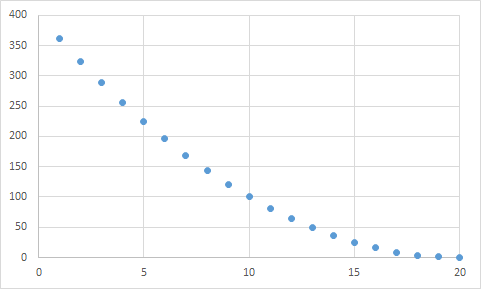
\includegraphics[scale=0.75]{satfun1}
\end{center}

\noindent
\textbf{Strange function} \hspace{.1in} This function assumes that for the voter the difference between two candidates from the top is the same as the difference between two candidates from the bottom, while differences between candidates from the middle of the preference order are much less significant. The function is given as follows:

\begin{gather}
	f(x) = \frac{x^{2}+x}{2} \\
	h = \frac{m}{2} \\
	d = f(h) \\
	\alpha(i) = \begin{cases} f(h-i+1)+d-1 : i<h \\ -f(i-h)+d : i \geq h \end{cases}
\end{gather}
\\

Example of function for $m = 20$:

\begin{center}
	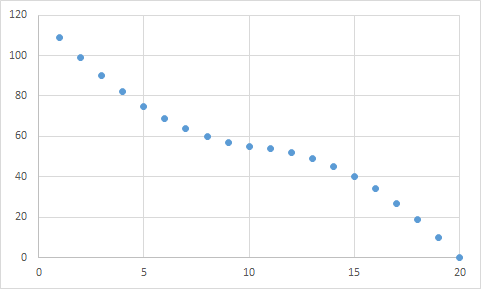
\includegraphics[scale=0.75]{satfun2}
\end{center}

\subsection{Summary}

Table below presents all generated test cases.

\begin{tabular}{r | c | c | c | c | c |}
	\# & alternatives count & agents count & winners count & generation model & satisfaction function \\
	\hline
	1 & \multirow{8}{*}{10} & \multirow{8}{*}{30} & \multirow{4}{*}{2} & \multirow{2}{*}{Polya} & Square \\
	2 & & & & & Strange \\
	\cline{5-6}
	3 & & & & \multirow{2}{*}{IC} & Square \\
	4 & & & & & Strange \\
	\cline{4-6}
	5 & & & \multirow{4}{*}{5} & \multirow{2}{*}{Polya} & Square \\
	6 & & & & & Strange \\
	\cline{5-6}
	7 & & & & \multirow{2}{*}{IC} & Square \\
	8 & & & & & Strange \\
	\hline
	9 & \multirow{8}{*}{50} & \multirow{8}{*}{400} & \multirow{4}{*}{10} & \multirow{2}{*}{Polya} & Square \\
	10 & & & & & Strange \\
	\cline{5-6}
	11 & & & & \multirow{2}{*}{IC} & Square \\
	12 & & & & & Strange \\
	\cline{4-6}
	13 & & & \multirow{4}{*}{25} & \multirow{2}{*}{Polya} & Square \\
	14 & & & & & Strange \\
	\cline{5-6}
	15 & & & & \multirow{2}{*}{IC} & Square \\
	16 & & & & & Strange \\
	\hline
	17 & \multirow{8}{*}{300} & \multirow{8}{*}{400} & \multirow{4}{*}{50} & \multirow{2}{*}{Polya} & Square \\
	18 & & & & & Strange \\
	\cline{5-6}
	19 & & & & \multirow{2}{*}{IC} & Square \\
	20 & & & & & Strange \\
	\cline{4-6}
	21 & & & \multirow{4}{*}{200} & \multirow{2}{*}{Polya} & Square \\
	22 & & & & & Strange \\
	\cline{5-6}
	23 & & & & \multirow{2}{*}{IC} & Square \\
	24 & & & & & Strange \\
	\hline
\end{tabular}
\\

\section{Test Methodology}

For each combination of problem size and generation model 100 files were generated independently. Algorithms were evaluated against all test files for each test case. We measured execution time and solution quality (total satisfaction) which was compared with brute-force (optimal) result for small instances and upper bound (total satisfaction if every agent has his top alternative assigned) for medium and large instances. Execution time and solution quality comparison with brute-force result or upper bound are presented as an average of 100 results (with standard deviation).
\\

All test cases were used for both Chamberlin-Courant and Monroe problems.

\section{Chamberlin-Courant Problem Evaluation}

In this section we present evaluation results for Chamberlin-Courant problem.

\subsection{Small instance}

Results for small instance ($n = 30$, $m = 10$). Results are compared to optimal results.
\\

Evaluated algorithms:
\begin{itemize}
	\item Algorithm C ($d = 10$)
	\item Algorithm C ($d = 15$)
	\item Algorithm R ($k = 100$)
	\item Algorithm GM
	\item Algorithm P
	\item Genetic Algorithm ($I = 15, c = 5$)
	\item Simulated Annealing ($T_{start} = 100, c = 0.1$)
\end{itemize}

Results for 2 winners:
\\

\begin{tabular}{| l | r | r | r | r |}
	\hline
	\multicolumn{5}{| c |}{$n = 30$, $m = 10$, $K = 2$, Square function} \\
	\hline
	\multirow{2}{*}{algorithm} & \multicolumn{2}{c |}{Polya} & \multicolumn{2}{c |}{IC} \\
	\cline{2-5}
	& \multicolumn{1}{c |}{time [ms]} & \multicolumn{1}{c |}{quality} & \multicolumn{1}{c |}{time [ms]} & \multicolumn{1}{c |}{quality} \\
	\hline
	C (10) & $0.66 \pm 0.12$ & $100.000 \pm 0.000 \%$ & $0.68 \pm 0.14$ & $100.000 \pm 0.000 \%$ \\
	\hline
	C (15) & $0.74 \pm 0.16$ & $100.000 \pm 0.000 \%$ & $0.74 \pm 0.14$ & $100.000 \pm 0.000 \%$ \\
	\hline
	R (100) & $0.75 \pm 0.14$ & $99.710 \pm 1.162 \%$ & $0.58 \pm 0.05$ & $99.479 \pm 1.470 \%$ \\
	\hline
	GM & $0.14 \pm 0.03$ & $99.992 \pm 0.055 \%$ & $0.10 \pm 0.02$ & $99.690 \pm 0.856 \%$ \\
	\hline
	P & $0.06 \pm 0.01$ & $87.964 \pm 8.825 \%$ & $0.05 \pm 0.02$ & $90.096 \pm 6.482 \%$ \\
	\hline
	GA (15, 5) & $0.68 \pm 0.14$ & $99.633 \pm 1.261 \%$ & $0.53 \pm 0.06$ & $99.505 \pm 1.555 \%$ \\
	\hline
	SA (100, 0.1) & $0.37 \pm 0.07$ & $98.603 \pm 2.375 \%$ & $0.28 \pm 0.04$ & $98.693 \pm 2.549 \%$ \\
	\hline
\end{tabular}

\vspace{16pt}

\begin{tabular}{| l | r | r | r | r |}
	\hline
	\multicolumn{5}{| c |}{$n = 30$, $m = 10$, $K = 2$, Strange function} \\
	\hline
	\multirow{2}{*}{algorithm} & \multicolumn{2}{c |}{Polya} & \multicolumn{2}{c |}{IC} \\
	\cline{2-5}
	& \multicolumn{1}{c |}{time [ms]} & \multicolumn{1}{c |}{quality} & \multicolumn{1}{c |}{time [ms]} & \multicolumn{1}{c |}{quality} \\
	\hline
	C (10) & $0.54 \pm 0.07$ & $100.000 \pm 0.000 \%$ & $0.56 \pm 0.15$ & $100.000 \pm 0.000 \%$ \\
	\hline
	C (15) & $0.56 \pm 0.06$ & $100.000 \pm 0.000 \%$ & $0.55 \pm 0.06$ & $100.000 \pm 0.000 \%$ \\
	\hline
	R (100) & $0.72 \pm 0.15$ & $99.718 \pm 1.021 \%$ & $0.59 \pm 0.07$ & $99.947 \pm 0.240 \%$ \\
	\hline
	GM & $0.16 \pm 0.03$ & $99.994 \pm 0.044 \%$ & $0.11 \pm 0.03$ & $99.414 \pm 1.375 \%$ \\
	\hline
	P & $0.06 \pm 0.01$ & $91.785 \pm 6.058 \%$ & $0.05 \pm 0.01$ & $93.725 \pm 4.245 \%$ \\
	\hline
	GA (15, 5) & $0.68 \pm 0.15$ & $99.910 \pm 0.383 \%$ & $0.52 \pm 0.05$ & $99.670 \pm 0.780 \%$ \\
	\hline
	SA (100, 0.1) & $0.32 \pm 0.05$ & $98.820 \pm 2.256 \%$ & $0.27 \pm 0.04$ & $99.144 \pm 1.778 \%$ \\
	\hline
\end{tabular}

\vspace{16pt}

Results for 5 winners:
\\

\begin{tabular}{| l | r | r | r | r |}
	\hline
	\multicolumn{5}{| c |}{$n = 30$, $m = 10$, $K = 5$, Square function} \\
	\hline
	\multirow{2}{*}{algorithm} & \multicolumn{2}{c |}{Polya} & \multicolumn{2}{c |}{IC} \\
	\cline{2-5}
	& \multicolumn{1}{c |}{time [ms]} & \multicolumn{1}{c |}{quality} & \multicolumn{1}{c |}{time [ms]} & \multicolumn{1}{c |}{quality} \\
	\hline
	C (10) & $1.67 \pm 0.30$ & $100.000 \pm 0.000 \%$ & $1.59 \pm 0.13$ & $99.993 \pm 0.073 \%$ \\
	\hline
	C (15) & $2.29 \pm 0.52$ & $100.000 \pm 0.000 \%$ & $2.41 \pm 0.48$ & $100.000 \pm 0.000 \%$ \\
	\hline
	R (100) & $0.95 \pm 0.09$ & $99.389 \pm 0.741 \%$ & $0.94 \pm 0.07$ & $99.218 \pm 0.842 \%$ \\
	\hline
	GM & $0.16 \pm 0.02$ & $99.980 \pm 0.108 \%$ & $0.16 \pm 0.01$ & $99.534 \pm 0.738 \%$ \\
	\hline
	P & $0.06 \pm 0.01$ & $91.789 \pm 4.927 \%$ & $0.06 \pm 0.01$ & $92.450 \pm 3.546 \%$ \\
	\hline
	GA (15, 5) & $0.94 \pm 0.04$ & $99.728 \pm 0.686 \%$ & $0.97 \pm 0.05$ & $99.349 \pm 1.014 \%$ \\
	\hline
	SA (100, 0.1) & $0.53 \pm 0.04$ & $98.185 \pm 1.550 \%$ & $0.53 \pm 0.03$ & $98.323 \pm 1.464 \%$ \\
	\hline
\end{tabular}

\vspace{16pt}

\begin{tabular}{| l | r | r | r | r |}
	\hline
	\multicolumn{5}{| c |}{$n = 30$, $m = 10$, $K = 5$, Strange function} \\
	\hline
	\multirow{2}{*}{algorithm} & \multicolumn{2}{c |}{Polya} & \multicolumn{2}{c |}{IC} \\
	\cline{2-5}
	& \multicolumn{1}{c |}{time [ms]} & \multicolumn{1}{c |}{quality} & \multicolumn{1}{c |}{time [ms]} & \multicolumn{1}{c |}{quality} \\
	\hline
	C (10) & $1.54 \pm 0.13$ & $100.000 \pm 0.000 \%$ & $1.68 \pm 0.45$ & $100.000 \pm 0.000 \%$ \\
	\hline
	C (15) & $2.35 \pm 0.64$ & $100.000 \pm 0.000 \%$ & $2.27 \pm 0.13$ & $100.000 \pm 0.000 \%$ \\
	\hline
	R (100) & $0.93 \pm 0.08$ & $99.331 \pm 0.768 \%$ & $0.94 \pm 0.08$ & $99.425 \pm 0.632 \%$ \\
	\hline
	GM & $0.16 \pm 0.02$ & $99.982 \pm 0.091 \%$ & $0.16 \pm 0.00$ & $99.672 \pm 0.615 \%$ \\
	\hline
	P & $0.06 \pm 0.01$ & $90.235 \pm 3.734 \%$ & $0.06 \pm 0.01$ & $94.353 \pm 2.656 \%$ \\
	\hline
	GA (15, 5) & $0.96 \pm 0.10$ & $99.710 \pm 0.607 \%$ & $0.99 \pm 0.06$ & $99.621 \pm 0.544 \%$ \\
	\hline
	SA (100, 0.1) & $0.54 \pm 0.04$ & $98.431 \pm 1.350 \%$ & $0.53 \pm 0.03$ & $98.741 \pm 0.959 \%$ \\
	\hline
\end{tabular}

\subsubsection{Conclusions}

Conclusions from small instance results:
\begin{enumerate}
	\item Results show no significant differences between Square and Strange satisfaction functions.
	\item Algorithm C seems to be the best one in the terms of solution quality. It returned an optimal solution for all cases except one, in which increasing number of stored functions ($d$) from 10 to 15 allowed it to return an optimal solution anyway.
	\item Algorithm GM is also returning very good results, although not optimal, while being much faster than Algorithm C. It remains to be seen how these algorithms behave in relation to each other for larger instances.
	\item Algorithm R performs surprisingly well, but for every case either Algorithm C or Algorithm GM is faster and gives better results.
	\item Algorithm P is the fastest one, but it also returns the worst results. It has very large standard deviation, which means that for some instances it returns much better result than average, but for some much worse.
	\item Genetic Algorithm and Simulated Annealing do not perform well, as they are both significantly slower than Algorithm GM, while returning worse results. For larger instances, we tried different input parameters to see if it makes these algorithms perform better.
	\item Results seem to be very similar for Polya and IC for such small instance. Only algorithm P performs better under IC, which is rather counter-intuitive. However, it may be caused by high standard deviation and therefore too small number of test files for this result to be representative.
\end{enumerate}

\subsection{Medium instance}

Results for medium instance ($n = 400$, $m = 50$). Results are compared to upper bound.
\\

Evaluated algorithms:
\begin{itemize}
	\item Algorithm C ($d = 10$)
	\item Algorithm C ($d = 15$)
	\item Algorithm R ($k = 100$)
	\item Algorithm GM
	\item Algorithm P
	\item Genetic Algorithm ($I = 100, c = 20$)
	\item Genetic Algorithm ($I = 200, c = 25$)
	\item Simulated Annealing ($T_{start} = 100, c = 0.01$)
	\item Simulated Annealing ($T_{start} = 100, c = 0.005$)
\end{itemize}

Results for 10 winners:
\\

\begin{tabular}{| l | r | r | r | r |}
	\hline
	\multicolumn{5}{| c |}{$n = 400$, $m = 50$, $K = 10$, Square function} \\
	\hline
	\multirow{2}{*}{algorithm} & \multicolumn{2}{c |}{Polya} & \multicolumn{2}{c |}{IC} \\
	\cline{2-5}
	& \multicolumn{1}{c |}{time [ms]} & \multicolumn{1}{c |}{quality} & \multicolumn{1}{c |}{time [ms]} & \multicolumn{1}{c |}{quality} \\
	\hline
	C (10) & $251.85 \pm 11.73$ & $96.517 \pm 0.553 \%$ & $267.20 \pm 9.65$ & $89.757 \pm 0.294 \%$ \\
	\hline
	C (15) & $379.52 \pm 9.60$ & $96.517 \pm 0.553 \%$ & $402.30 \pm 9.43$ & $89.769 \pm 0.286 \%$ \\
	\hline
	R (100) & $938.14 \pm 11.43$ & $94.589 \pm 0.727 \%$ & $941.29 \pm 12.78$ & $88.540 \pm 0.224 \%$ \\
	\hline
	GM & $25.45 \pm 0.96$ & $96.508 \pm 0.591 \%$ & $27.24 \pm 2.11$ & $89.494 \pm 0.377 \%$ \\
	\hline
	P & $2.62 \pm 0.07$ & $89.795 \pm 2.308 \%$ & $2.68 \pm 0.22$ & $86.599 \pm 0.711 \%$ \\
	\hline
	GA (100, 20) & $696.82 \pm 15.81$ & $96.256 \pm 0.563 \%$ & $761.59 \pm 11.25$ & $89.412 \pm 0.315 \%$ \\
	\hline
	GA (200, 25) & $1723.27 \pm 23.67$ & $96.404 \pm 0.553 \%$ & $1894.81 \pm 19.53$ & $89.562 \pm 0.292 \%$ \\
	\hline
	SA (100, 0.01) & $169.32 \pm 7.39$ & $93.589 \pm 0.866 \%$ & $169.55 \pm 7.59$ & $88.132 \pm 0.302 \%$ \\
	\hline
	SA (100, 0.005) & $335.91 \pm 7.52$ & $94.013 \pm 0.911 \%$ & $334.44 \pm 6.37$ & $88.207 \pm 0.234 \%$ \\
	\hline
\end{tabular}

\vspace{16pt}

\begin{tabular}{| l | r | r | r | r |}
	\hline
	\multicolumn{5}{| c |}{$n = 400$, $m = 50$, $K = 10$, Strange function} \\
	\hline
	\multirow{2}{*}{algorithm} & \multicolumn{2}{c |}{Polya} & \multicolumn{2}{c |}{IC} \\
	\cline{2-5}
	& \multicolumn{1}{c |}{time [ms]} & \multicolumn{1}{c |}{quality} & \multicolumn{1}{c |}{time [ms]} & \multicolumn{1}{c |}{quality} \\
	\hline
	C (10) & $251.14 \pm 9.65$ & $96.733 \pm 0.510 \%$ & $266.23 \pm 9.37$ & $90.719 \pm 0.255 \%$ \\
	\hline
	C (15) & $380.68 \pm 10.18$ & $96.733 \pm 0.510 \%$ & $404.76 \pm 11.29$ & $90.731 \pm 0.247 \%$ \\
	\hline
	R (100) & $941.99 \pm 16.86$ & $95.084 \pm 0.624 \%$ & $951.27 \pm 15.43$ & $89.698 \pm 0.188 \%$ \\
	\hline
	GM & $25.56 \pm 1.46$ & $96.725 \pm 0.516 \%$ & $27.16 \pm 1.86$ & $90.529 \pm 0.323 \%$ \\
	\hline
	P & $2.61 \pm 0.07$ & $90.769 \pm 1.985 \%$ & $2.68 \pm 0.28$ & $88.062 \pm 0.600 \%$ \\
	\hline
	GA (100, 20) & $696.42 \pm 15.04$ & $96.518 \pm 0.526 \%$ & $760.18 \pm 12.71$ & $90.423 \pm 0.247 \%$ \\
	\hline
	GA (200, 25) & $1738.66 \pm 27.14$ & $96.631 \pm 0.515 \%$ & $1922.78 \pm 24.20$ & $90.554 \pm 0.261 \%$ \\
	\hline
	SA (100, 0.01) & $167.29 \pm 5.80$ & $93.988 \pm 0.739 \%$ & $167.73 \pm 7.18$ & $89.329 \pm 0.292 \%$ \\
	\hline
	SA (100, 0.005) & $338.42 \pm 10.02$ & $94.450 \pm 0.719 \%$ & $342.32 \pm 11.21$ & $89.450 \pm 0.230 \%$ \\
	\hline
\end{tabular}

\vspace{16pt}

\newpage

Results for 25 winners:
\\

\begin{tabular}{| l | r | r | r | r |}
	\hline
	\multicolumn{5}{| c |}{$n = 400$, $m = 50$, $K = 25$, Square function} \\
	\hline
	\multirow{2}{*}{algorithm} & \multicolumn{2}{c |}{Polya} & \multicolumn{2}{c |}{IC} \\
	\cline{2-5}
	& \multicolumn{1}{c |}{time [ms]} & \multicolumn{1}{c |}{quality} & \multicolumn{1}{c |}{time [ms]} & \multicolumn{1}{c |}{quality} \\
	\hline
	C (10) & $541.20 \pm 12.76$ & $99.374 \pm 0.015 \%$ & $569.84 \pm 12.51$ & $97.585 \pm 0.119 \%$ \\
	\hline
	C (15) & $832.17 \pm 16.83$ & $99.374 \pm 0.015 \%$ & $869.71 \pm 14.88$ & $97.597 \pm 0.118 \%$ \\
	\hline
	R (100) & $2094.20 \pm 15.70$ & $98.574 \pm 0.204 \%$ & $2142.40 \pm 22.10$ & $97.041 \pm 0.084 \%$ \\
	\hline
	GM & $51.70 \pm 3.53$ & $99.373 \pm 0.146 \%$ & $54.80 \pm 3.58$ & $97.518 \pm 0.126 \%$ \\
	\hline
	P & $4.40 \pm 0.14$ & $96.740 \pm 0.855 \%$ & $4.42 \pm 0.09$ & $96.235 \pm 0.255 \%$ \\
	\hline
	GA (100, 20) & $1652.20 \pm 28.08$ & $99.138 \pm 0.183 \%$ & $1781.69 \pm 21.33$ & $97.335 \pm 0.102 \%$ \\
	\hline
	GA (200, 25) & $4096.02 \pm 60.15$ & $99.188 \pm 0.179 \%$ & $4483.16 \pm 43.37$ & $97.383 \pm 0.100 \%$ \\
	\hline
	SA (100, 0.01) & $399.24 \pm 8.47$ & $98.170 \pm 0.302 \%$ & $399.77 \pm 8.48$ & $96.859 \pm 0.113 \%$ \\
	\hline
	SA (100, 0.005) & $813.16 \pm 15.30$ & $98.326 \pm 0.252 \%$ & $813.26 \pm 14.00$ & $96.898 \pm 0.098 \%$ \\
	\hline
\end{tabular}

\vspace{16pt}

\begin{tabular}{| l | r | r | r | r |}
	\hline
	\multicolumn{5}{| c |}{$n = 400$, $m = 50$, $K = 25$, Strange function} \\
	\hline
	\multirow{2}{*}{algorithm} & \multicolumn{2}{c |}{Polya} & \multicolumn{2}{c |}{IC} \\
	\cline{2-5}
	& \multicolumn{1}{c |}{time [ms]} & \multicolumn{1}{c |}{quality} & \multicolumn{1}{c |}{time [ms]} & \multicolumn{1}{c |}{quality} \\
	\hline
	C (10) & $540.44 \pm 12.59$ & $99.404 \pm 0.138 \%$ & $567.23 \pm 12.07$ & $97.726 \pm 0.108 \%$ \\
	\hline
	C (15) & $831.26 \pm 18.11$ & $99.404 \pm 0.138 \%$ & $863.77 \pm 16.02$ & $97.732 \pm 0.103 \%$ \\
	\hline
	R (100) & $2136.59 \pm 23.57$ & $98.667 \pm 0.186 \%$ & $2091.77 \pm 16.60$ & $97.214 \pm 0.085 \%$ \\
	\hline
	GM & $51.68 \pm 2.23$ & $99.403 \pm 0.138 \%$ & $54.74 \pm 3.07$ & $97.662 \pm 0.118 \%$ \\
	\hline
	P & $4.39 \pm 0.25$ & $96.939 \pm 0.790 \%$ & $4.45 \pm 0.54$ & $96.472 \pm 0.233 \%$ \\
	\hline
	GA (100, 20) & $1649.14 \pm 28.84$ & $99.180 \pm 0.179 \%$ & $1769.20 \pm 19.84$ & $97.491 \pm 0.096 \%$ \\
	\hline
	GA (200, 25) & $4104.78 \pm 61.44$ & $99.227 \pm 0.172 \%$ & $4422.15 \pm 27.53$ & $97.548 \pm 0.099 \%$ \\
	\hline
	SA (100, 0.01) & $397.18 \pm 8.62$ & $98.280 \pm 0.268 \%$ & $396.13 \pm 6.25$ & $97.034 \pm 0.111 \%$ \\
	\hline
	SA (100, 0.005) & $799.15 \pm 11.14$ & $98.397 \pm 0.233 \%$ & $799.15 \pm 9.75$ & $97.090 \pm 0.105 \%$ \\
	\hline
\end{tabular}

\newpage

\subsubsection{Conclusions}

Conclusions from medium instance results:
\begin{enumerate}
	\item Solution quality compared to upper bound is generally a bit better for Strange satisfaction function. This is because for top alternatives Square function decreases faster compared to the first alternative (see chart below), so algorithms score is relatively worse when selecting second or third alternative in the preference order.
	\begin{center}
		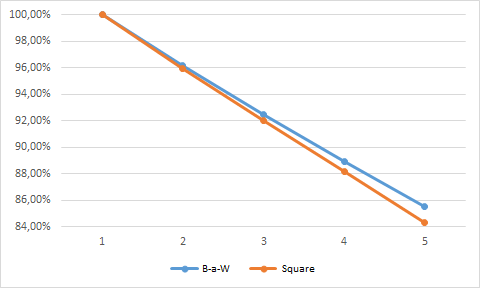
\includegraphics[scale=0.75]{satfuncomp1}
	\end{center}
	\item The difference between Polya and IC is clearly visible now (Polya could still be too random for smaller instance to see the diference). It is much easier to find a solution close to an upper bound for a Polya generation model, as there is a group of alternatives that are ranked high by most agents, while IC is totally random.
	\item Algorithm C is still the best algorithm in terms of solution quality. For Polya, it finds solutions very close to an upper bound, especially with $K = 25$, which means that most agents have their favourite alternative assigned. For IC using $d = 15$ instead of $d = 10$ slightly improves the solution quality, so if we seek the best solution possible, setting higher $d$ is reasonable.
	\item Algorithm GM performs excellently, attaining only slightly lower solution quality than Algorithm C in most cases, while executing much faster.
	\item Algorithm P is still very fast, and additionally standard deviation of its quality is acceptable for this problem size (there should be no instances for which the solution quality is much worse than average). Quality is much lower than for Algorithms C or GM, but if we need a decent solution that does not have to be optimal and we want to calculate it fast, this algorithm may be used.
	\item Algorithm R does not seem to be useful for this problem size. It executes longer than Algorithm C and returns much worse results.
	\item Genetic Algorithm generates solutions of very good quality (comparable to Algorithm GM), but executes much too long to be useful in both tested configurations. Simulated Annealing also seems to be useless, as Algorithm GM executes much faster and gives better results.
\end{enumerate}

\subsection{Large instance}

Results for large instance ($n = 400$, $m = 300$). Results are compared to upper bound.
\\

Evaluated algorithms:
\begin{itemize}
	\item Algorithm C ($d = 10$)
	\item Algorithm C ($d = 15$)
	\item Algorithm R ($k = 100$)
	\item Algorithm GM
	\item Algorithm P
	\item Genetic Algorithm ($I = 100, c = 20$)
	\item Genetic Algorithm ($I = 200, c = 25$)
	\item Simulated Annealing ($T_{start} = 100, c = 0.01$)
	\item Simulated Annealing ($T_{start} = 100, c = 0.005$)
\end{itemize}

\newpage

Results for 50 winners:
\\

\begin{tabular}{| l | r | r | r | r |}
	\hline
	\multicolumn{5}{| c |}{$n = 400$, $m = 300$, $K = 50$, Square function} \\
	\hline
	\multirow{2}{*}{algorithm} & \multicolumn{2}{c |}{Polya} & \multicolumn{2}{c |}{IC} \\
	\cline{2-5}
	& \multicolumn{1}{c |}{time [s]} & \multicolumn{1}{c |}{quality} & \multicolumn{1}{c |}{time [s]} & \multicolumn{1}{c |}{quality} \\
	\hline
	C (10) & $15.66 \pm 0.11$ & $99.418 \pm 0.051 \%$ & $16.33 \pm 0.10$ & $98.466 \pm 0.056 \%$ \\
	\hline
	C (15) & $24.12 \pm 0.12$ & $99.420 \pm 0.051 \%$ & $25.04 \pm 0.14$ & $98.472 \pm 0.061 \%$ \\
	\hline
	R (100) & $0.337 \pm 0.011$ & $97.787 \pm 0.140 \%$ & $0.337 \pm 0.011$ & $97.197 \pm 0.075 \%$ \\
	\hline
	GM & $1.46 \pm 0.02$ & $99.412 \pm 0.052 \%$ & $1.53 \pm 0.02$ & $98.400 \pm 0.071 \%$ \\
	\hline
	P & $0.0585 \pm 0.0045$ & $97.029 \pm 0.416 \%$ & $0.0588 \pm 0.0049$ & $96.804 \pm 0.154 \%$ \\
	\hline
	GA (100, 20) & $6.96 \pm 0.11$ & $99.039 \pm 0.084 \%$ & $8.41 \pm 0.05$ & $97.822 \pm 0.073 \%$ \\
	\hline
	GA (200, 25) & $16.81 \pm 0.29$ & $99.125 \pm 0.069 \%$ & $20,88 \pm 0.14$ & $97.927 \pm 0.062 \%$ \\
	\hline
	SA (100, 0.01) & $1.91 \pm 0.03$ & $97.662 \pm 0.213 \%$ & $1.92 \pm 0.02$ & $97.197 \pm 0.087 \%$ \\
	\hline
	SA (100, 0.005) & $3.81 \pm 0.05$ & $97.794 \pm 0.172 \%$ & $3.85 \pm 0.03$ & $97.221 \pm 0.082 \%$ \\
	\hline
\end{tabular}

\vspace{16pt}

\begin{tabular}{| l | r | r | r | r |}
	\hline
	\multicolumn{5}{| c |}{$n = 400$, $m = 300$, $K = 50$, Strange function} \\
	\hline
	\multirow{2}{*}{algorithm} & \multicolumn{2}{c |}{Polya} & \multicolumn{2}{c |}{IC} \\
	\cline{2-5}
	& \multicolumn{1}{c |}{time [s]} & \multicolumn{1}{c |}{quality} & \multicolumn{1}{c |}{time [s]} & \multicolumn{1}{c |}{quality} \\
	\hline
	C (10) & $15.68 \pm 0.16$ & $99.425 \pm 0.050 \%$ & $16.32 \pm 0.10$ & $98.495 \pm 0.059 \%$ \\
	\hline
	C (15) & $24.07 \pm 0.14$ & $99.426 \pm 0.050 \%$ & $25.05 \pm 0.13$ & $98.502 \pm 0.060 \%$ \\
	\hline
	R (100) & $0.329 \pm 0.002$ & $97.838 \pm 0.129 \%$ & $0.329 \pm 0.002$ & $97.264 \pm 0.073 \%$ \\
	\hline
	GM & $1.42 \pm 0.01$ & $99.419 \pm 0.052 \%$ & $1.49 \pm 0.01$ & $98.438 \pm 0.075 \%$ \\
	\hline
	P & $0.0575 \pm 0.0006$ & $97.098 \pm 0.400 \%$ & $0.0583 \pm 0.005$ & $96.881 \pm 0.148 \%$ \\
	\hline
	GA (100, 20) & $6.79 \pm 0.10$ & $99.054 \pm 0.081 \%$ & $8.25 \pm 0.03$ & $97.872 \pm 0.069 \%$ \\
	\hline
	GA (200, 25) & $16.61 \pm 0.23$ & $99.131 \pm 0.073 \%$ & $20.50 \pm 0.42$ & $97.952 \pm 0.059 \%$ \\
	\hline
	SA (100, 0.01) & $1.89 \pm 0.03$ & $97.741 \pm 0.197 \%$ & $1.89 \pm 0.01$ & $97.239 \pm 0.092 \%$ \\
	\hline
	SA (100, 0.005) & $3.77 \pm 0.04$ & $97.840 \pm 0.175 \%$ & $3.78 \pm 0.01$ & $97.286 \pm 0.072 \%$ \\
	\hline
\end{tabular}

\vspace{16pt}

\newpage

Results for 200 winners:
\\

\begin{tabular}{| l | r | r | r | r |}
	\hline
	\multicolumn{5}{| c |}{$n = 400$, $m = 300$, $K = 200$, Square function} \\
	\hline
	\multirow{2}{*}{algorithm} & \multicolumn{2}{c |}{Polya} & \multicolumn{2}{c |}{IC} \\
	\cline{2-5}
	& \multicolumn{1}{c |}{time [s]} & \multicolumn{1}{c |}{quality} & \multicolumn{1}{c |}{time [s]} & \multicolumn{1}{c |}{quality} \\
	\hline
	C (10) & $50.19 \pm 0.38$ & $100.000 \pm 0.000 \%$ & $50.54 \pm 0.27$ & $99.9536 \pm 0.0099 \%$ \\
	\hline
	C (15) & $79.44 \pm 0.60$ & $100.000 \pm 0.000 \%$ & $81.67 \pm 0.62$ & $99.9537 \pm 0.0097 \%$ \\
	\hline
	R (100) & $1.29 \pm 0.01$ & $99.776 \pm 0.016 \%$ & $1.29 \pm 0.00$ & $99.737 \pm 0.011 \%$ \\
	\hline
	GM & $4.04 \pm 0.02$ & $100.000 \pm 0.000 \%$ & $4.00 \pm 0.01$ & $99.952 \pm 0.010 \%$ \\
	\hline
	P & $0.134 \pm 0.002$ & $99.669 \pm 0.044 \%$ & $0.134 \pm 0.002$ & $99.672 \pm 0.031 \%$ \\
	\hline
	GA (100, 20) & $27.20 \pm 0.97$ & $100.000 \pm 0.000 \%$ & $30.67 \pm 0.08$ & $99.950 \pm 0.015 \%$ \\
	\hline
	GA (200, 25) & $67.72 \pm 2.41$ & $100.000 \pm 0.000 \%$ & $76.45 \pm 0.21$ & $99.953 \pm 0.014 \%$ \\
	\hline
	SA (100, 0.01) & $7.08 \pm 0.04$ & $99.757 \pm 0.021 \%$ & $7.05 \pm 0.02$ & $99.724 \pm 0.017 \%$ \\
	\hline
	SA (100, 0.005) & $14.16 \pm 0.06$ & $99.773 \pm 0.024 \%$ & $14.10 \pm 0.03$ & $99.736 \pm 0.014 \%$ \\
	\hline
\end{tabular}

\vspace{16pt}

\begin{tabular}{| l | r | r | r | r |}
	\hline
	\multicolumn{5}{| c |}{$n = 400$, $m = 300$, $K = 200$, Strange function} \\
	\hline
	\multirow{2}{*}{algorithm} & \multicolumn{2}{c |}{Polya} & \multicolumn{2}{c |}{IC} \\
	\cline{2-5}
	& \multicolumn{1}{c |}{time [s]} & \multicolumn{1}{c |}{quality} & \multicolumn{1}{c |}{time [s]} & \multicolumn{1}{c |}{quality} \\
	\hline
	C (10) & $49.33 \pm 0.35$ & $100.000 \pm 0.000 \%$ & $50.04 \pm 0.20$ & $99.9538 \pm 0.0091 \%$ \\
	\hline
	C (15) & $78.57 \pm 0.50$ & $100.000 \pm 0.000 \%$ & $80.79 \pm 0.33$ & $99.9542 \pm 0.0097 \%$ \\
	\hline
	R (100) & $1.30 \pm 0.00$ & $99.776 \pm 0.014 \%$ & $1.30 \pm 0.00$ & $99.741 \pm 0.011 \%$ \\
	\hline
	GM & $4.05 \pm 0.01$ & $100.000 \pm 0.000 \%$ & $4.00 \pm 0.01$ & $99.953 \pm 0.010 \%$ \\
	\hline
	P & $0.134 \pm 0.001$ & $99.672 \pm 0.043 \%$ & $0.134 \pm 0.001$ & $99.676 \pm 0.031 \%$ \\
	\hline
	GA (100, 20) & $27.29 \pm 0.97$ & $100.000 \pm 0.000 \%$ & $30.77 \pm 0.05$ & $99.950 \pm 0.015 \%$ \\
	\hline
	GA (200, 25) & $67.79 \pm 2.41$ & $100.000 \pm 0.000 \%$ & $77.74 \pm 0.41$ & $99.954 \pm 0.014 \%$ \\
	\hline
	SA (100, 0.01) & $7.11 \pm 0.04$ & $99.755 \pm 0.026 \%$ & $7.24 \pm 0.05$ & $99.727 \pm 0.017 \%$ \\
	\hline
	SA (100, 0.005) & $14.22 \pm 0.07$ & $99.773 \pm 0.022 \%$ & $14.32 \pm 0.11$ & $99.736 \pm 0.016 \%$ \\
	\hline
\end{tabular}

\subsubsection{Conclusions}

Conclusions from large instance results:
\begin{enumerate}
	\item These test cases turned out to be very easy for tested algorithms - all solutions are of very high quality compared to upper bound. The reason of this is very high number of winners, which allows many agents to have their favourite alternative assigned, even for data generated with IC model. For Polya and 200 winners, many algorithms always return an optimal solution which has the same total satisfaction as upper bound - allowing 200 out of 300 candidates to win and using Polya model allows for every agent to be maximally satisfied in virtually every case.
	\item Relation between Algorithm C, Algorithm GM and Algorithm P remains the same as for the middle instance.
	\item For such large data sets, Algorithm R may become an option, as it runs relatively fast (not as fast as Algorithm P though) and returns solution of quality between Algorithm GM and Algorithm R. It is possible that this algorithm gets relatively better for even larger data sets.
	\item Genetic Algorithm and Simulated Annealing are not a viable option for small number of winners ($K = 50$), as they both return worse results than Algorithm GM and they run slower. However, Genetic Algorithm may be useful for large data sets where there is a lot of winners. For $K = 200$, it becomes similar to Algorithm GM in means of both execution time and solution quality.
\end{enumerate}

\subsection{Conclusions summary}

These are final conclusions regarding evaluation of algorithms for Chamberlin-Courant Problem based on all executed test cases.

\begin{enumerate}
	\item There is no significant difference between results for Square and Strange satisfaction functions. It seems that the most important part of the satisfaction function is near the top of the preference order, because middle and bottom alternatives are rarely selected and differences between them are not very important, and both Square and Strange functions are similar for the top alternatives. Results could be much different for some kind of exponential function.
	\item Algorithm C and Algorithm GM are viable for every tested case. One should use Algorithm C to get solution with the best quality possible (potentially increasing input parameter $d$ for a chance to find an even better solution). Algorithm GM always returns slightly weaker result than Algorithm C, but it runs much faster, so it may be used as a compromise between execution time and solution quality.
	\item Algorithm P returns substantially weaker solutions than Algorithm GM, but it runs extremely fast. It may be used if solution does not have to be good but not necessarily close to optimal (e.g., in recommendation systems), but there is a need to obtain it as fast as possible. This algorithm should not be used for small data sets, because the solution may be of very low quality, but this should not be a problem, because for small instances Algorithms GM runs very fast too.
	\item For large cases, Algorithm R can provide good results with moderate execution time. However, due to high level of randomization, this algorithm should only be used to supplement another one, so it can possibly find a better solution.
	\item It is possible that Genetic Algorithm may be a good option for large cases with high winner count, but it requires further research.
\end{enumerate}

\section{Monroe Problem Evaluation}

In this section we present evaluation results for Monroe problem.

\subsection{Small instance}

Results for small instance ($n = 30$, $m = 10$). Results are compared to optimal results.
\\

Evaluated algorithms:
\begin{itemize}
	\item Algorithm A
	\item Algorithm B
	\item Algorithm C ($d = 10$)
	\item Algorithm C ($d = 15$)
	\item Algorithm R ($k = 100$)
	\item Algorithm AR ($e = 0.215$, $\lambda = 0.75$)
	\item Algorithm AR ($e = 0.015$, $\lambda = 0.9$)
	\item Algorithm GM
	\item Genetic Algorithm ($I = 15, c = 5$)
	\item Simulated Annealing ($T_{start} = 100, c = 0.1$)
\end{itemize}

\newpage

Results for 2 winners:
\\

\begin{tabular}{| l | r | r | r | r |}
	\hline
	\multicolumn{5}{| c |}{$n = 30$, $m = 10$, $K = 2$, Square function} \\
	\hline
	\multirow{2}{*}{algorithm} & \multicolumn{2}{c |}{Polya} & \multicolumn{2}{c |}{IC} \\
	\cline{2-5}
	& \multicolumn{1}{c |}{time [ms]} & \multicolumn{1}{c |}{quality} & \multicolumn{1}{c |}{time [ms]} & \multicolumn{1}{c |}{quality} \\
	\hline
	A & $0.18 \pm 0.03$ & $95.320 \pm 2.247 \%$ & $0.18 \pm 0.02$ & $94.738 \pm 2.321 \%$ \\
	\hline
	B & $0.61 \pm 0.08$ & $99.457 \pm 1.296 \%$ & $0.77 \pm 0.75$ & $99.046 \pm 1.710 \%$ \\
	\hline
	C (10) & $5.26 \pm 0.57$ & $100.000 \pm 0.000 \%$ & $5.36 \pm 0.88$ & $99.9967 \pm 0.0271 \%$ \\
	\hline
	C (15) & $7.39 \pm 0.57$ & $100.000 \pm 0.000 \%$ & $7.56 \pm 0.83$ & $99.9994 \pm 0.0063 \%$ \\
	\hline
	R (100) & $44.60 \pm 6.59$ & $99.376 \pm 2.374 \%$ & $43.26 \pm 4.16$ & $99.522 \pm 1.428 \%$ \\
	\hline
	AR (0.215, 0.75) & $20.75 \pm 2.29$ & $100.000 \pm 0.000 \%$ & $18.90 \pm 0.23$ & $100.000 \pm 0.000 \%$ \\
	\hline
	AR (0.015, 0.9) & $24.18 \pm 4.62$ & $100.000 \pm 0.000 \%$ & $21.90 \pm 5.97$ & $100.000 \pm 0.000 \%$ \\
	\hline
	GM & $6.46 \pm 1.22$ & $100.000 \pm 0.000 \%$ & $6.13 \pm 0.91$ & $99.833 \pm 0.640 \%$ \\
	\hline
	GA (15, 5) & $34.84 \pm 3.87$ & $99.352 \pm 2.259 \%$ & $34.97 \pm 4.21$ & $99.153 \pm 2.040 \%$ \\
	\hline
	SA (100, 0.1) & $19.11 \pm 0.68$ & $98.053 \pm 3.442 \%$ & $19.07 \pm 0.71$ & $98.482 \pm 2.579 \%$ \\
	\hline
\end{tabular}

\vspace{16pt}

\begin{tabular}{| l | r | r | r | r |}
	\hline
	\multicolumn{5}{| c |}{$n = 30$, $m = 10$, $K = 2$, Strange function} \\
	\hline
	\multirow{2}{*}{algorithm} & \multicolumn{2}{c |}{Polya} & \multicolumn{2}{c |}{IC} \\
	\cline{2-5}
	& \multicolumn{1}{c |}{time [ms]} & \multicolumn{1}{c |}{quality} & \multicolumn{1}{c |}{time [ms]} & \multicolumn{1}{c |}{quality} \\
	\hline
	A & $0.26 \pm 0.62$ & $96.872 \pm 1.604 \%$ & $0.19 \pm 0.04$ & $95.500 \pm 1.679 \%$ \\
	\hline
	B & $0.61 \pm 0.08$ & $99.581 \pm 1.019 \%$ & $0.61 \pm 0.08$ & $99.214 \pm 1.176 \%$ \\
	\hline
	C (10) & $5.41 \pm 0.77$ & $100.000 \pm 0.000 \%$ & $5.27 \pm 0.39$ & $99.980 \pm 0.152 \%$ \\
	\hline
	C (15) & $7.50 \pm 0.97$ & $100.000 \pm 0.000 \%$ & $7.63 \pm 1.42$ & $99.994 \pm 0.0062 \%$ \\
	\hline
	R (100) & $42.71 \pm 3.24$ & $99.545 \pm 2.078 \%$ & $43.32 \pm 1.69$ & $99.830 \pm 0.625 \%$ \\
	\hline
	AR (0.215, 0.75) & $22.14 \pm 5.08$ & $100.000 \pm 0.000 \%$ & $22.55 \pm 5.37$ & $100.000 \pm 0.000 \%$ \\
	\hline
	AR (0.015, 0.9) & $21.90 \pm 4.91$ & $100.000 \pm 0.000 \%$ & $22.62 \pm 5.53$ & $100.000 \pm 0.000 \%$ \\
	\hline
	GM & $5.94 \pm 0.62$ & $100.000 \pm 0.000 \%$ & $5.96 \pm 0.39$ & $99.847 \pm 0.524 \%$ \\
	\hline
	GA (15, 5) & $34.90 \pm 2.59$ & $99.662 \pm 1.274 \%$ & $35.40 \pm 4.34$ & $99.546 \pm 1.256 \%$ \\
	\hline
	SA (100, 0.1) & $19.97 \pm 2.94$ & $98.416 \pm 2.649 \%$ & $19.57 \pm 1.23$ & $99.161 \pm 1.692 \%$ \\
	\hline
\end{tabular}

\vspace{16pt}

\newpage

Results for 5 winners:
\\

\begin{tabular}{| l | r | r | r | r |}
	\hline
	\multicolumn{5}{| c |}{$n = 30$, $m = 10$, $K = 5$, Square function} \\
	\hline
	\multirow{2}{*}{algorithm} & \multicolumn{2}{c |}{Polya} & \multicolumn{2}{c |}{IC} \\
	\cline{2-5}
	& \multicolumn{1}{c |}{time [ms]} & \multicolumn{1}{c |}{quality} & \multicolumn{1}{c |}{time [ms]} & \multicolumn{1}{c |}{quality} \\
	\hline
	A & $0.25 \pm 0.02$ & $94.065 \pm 2.307 \%$ & $0.28 \pm 0.09$ & $95.567 \pm 2.081 \%$ \\
	\hline
	B & $0.91 \pm 0.30$ & $99.296 \pm 1.231 \%$ & $0.81 \pm 0.06$ & $99.017 \pm 1.443 \%$ \\
	\hline
	C (10) & $7.78 \pm 1.64$ & $99.991 \pm 0.070 \%$ & $7.77 \pm 1.01$ & $99.918 \pm 0.366 \%$ \\
	\hline
	C (15) & $11.43 \pm 1.97$ & $100.000 \pm 0.000 \%$ & $11.56 \pm 1.56$ & $99.974 \pm 0.112 \%$ \\
	\hline
	R (100) & $55.91 \pm 5.30$ & $97.678 \pm 2.753 \%$ & $55.28 \pm 4.34$ & $99.014 \pm 1.201 \%$ \\
	\hline
	AR (0.215, 0.75) & $137.13 \pm 5.69$ & $100.000 \pm 0.000 \%$ & $136.24 \pm 6.32$ & $100.000 \pm 0.000 \%$ \\
	\hline
	AR (0.015, 0.9) & $154.83 \pm 25.07$ & $100.000 \pm 0.000 \%$ & $153.26 \pm 23.78$ & $100.000 \pm 0.000 \%$ \\
	\hline
	GM & $11.20 \pm 1.23$ & $99.946 \pm 0.240 \%$ & $11.41 \pm 1.94$ & $99.841 \pm 0.392 \%$ \\
	\hline
	GA (15, 5) & $44.28 \pm 4.15$ & $99.110 \pm 1.819 \%$ & $45.07 \pm 6.11$ & $99.276 \pm 1.158 \%$ \\
	\hline
	SA (100, 0.1) & $24.49 \pm 1.76$ & $95.158 \pm 3.961 \%$ & $24.62 \pm 2.86$ & $98.022 \pm 1.707 \%$ \\
	\hline
\end{tabular}

\vspace{16pt}

\begin{tabular}{| l | r | r | r | r |}
	\hline
	\multicolumn{5}{| c |}{$n = 30$, $m = 10$, $K = 5$, Strange function} \\
	\hline
	\multirow{2}{*}{algorithm} & \multicolumn{2}{c |}{Polya} & \multicolumn{2}{c |}{IC} \\
	\cline{2-5}
	& \multicolumn{1}{c |}{time [ms]} & \multicolumn{1}{c |}{quality} & \multicolumn{1}{c |}{time [ms]} & \multicolumn{1}{c |}{quality} \\
	\hline
	A & $0.26 \pm 0.01$ & $96.012 \pm 0.163 \%$ & $0.27 \pm 0.03$ & $96.864 \pm 1.589 \%$ \\
	\hline
	B & $0.79 \pm 0.07$ & $99.390 \pm 1.017 \%$ & $0.80 \pm 0.09$ & $99.251 \pm 0.997 \%$ \\
	\hline
	C (10) & $8.18 \pm 1.87$ & $99.994 \pm 0.063 \%$ & $7.83 \pm 1.06$ & $99.939 \pm 0.237 \%$ \\
	\hline
	C (15) & $11.37 \pm 2.00$ & $99.989 \pm 0.080 \%$ & $11.04 \pm 0.48$ & $99.955 \pm 0.209 \%$ \\
	\hline
	R (100) & $55.31 \pm 4.24$ & $98.508 \pm 1.602 \%$ & $54.57 \pm 4.17$ & $99.217 \pm 0.849 \%$ \\
	\hline
	AR (0.215, 0.75) & $160.17 \pm 28.16$ & $100.000 \pm 0.000 \%$ & $156.45 \pm 26.68$ & $100.000 \pm 0.000 \%$ \\
	\hline
	AR (0.015, 0.9) & $157.34 \pm 26.41$ & $100.000 \pm 0.000 \%$ & $159.08 \pm 29.08$ & $100.000 \pm 0.000 \%$ \\
	\hline
	GM & $10.96 \pm 1.07$ & $99.971 \pm 0.158 \%$ & $11.15 \pm 1.74$ & $99.921 \pm 0.200 \%$ \\
	\hline
	GA (15, 5) & $44.08 \pm 4.53$ & $99.458 \pm 1.048 \%$ & $44.45 \pm 4.90$ & $99.601 \pm 0.715 \%$ \\
	\hline
	SA (100, 0.1) & $24.84 \pm 3.14$ & $96.261 \pm 2.710 \%$ & $24.70 \pm 2.93$ & $98.591 \pm 1.111 \%$ \\
	\hline
\end{tabular}

\subsubsection{Conclusions}

Conclusions from small instance results:
\begin{enumerate}
	\item For most cases algorithms generally return a bit higher satisfaction for the Strange function than for the Square function. It is caused by the fact that Square function is decreasing relatively faster for top alternatives (as described in section 5.4.2.1).
	\item Algorithm AR gives the best quality of solution among tested algorithms for every case (it always returns an optimal solution), but it is very slow (extremely slow for 5 winners case). It remains to be seen it is viable for use with larger problem instances.
	\item Algorithm C returns almost as good quality of solution as Algorithm AR and is much faster. For this problem size, it often returns an optimal solution, or the one very close to optimal. Increasing number of stored functions ($d$) can improve the result slightly.
	\item Execution times for Algorithm GM are very similar to Algorithm C and they are only of slightly lower quality. However, execution times are expected to rise fast when problem size is increased, because this algorithm requires many min-flow/max-cost function calls, which are very time-consuming.
	\item Quality of solution generated by Algorithm B is always significantly lower than the one generated by Algorithm C, but the algorithm itself is much faster (by one order of magnitude).
	\item For this problem size, Algorithm A is the fastest algorithm, but its quality of solution is very low.
	\item Algorithm R is not a good choice for this problem size, because it runs much longer than Algorithm C and returns worse results.
	\item Genetic Algorithm and Simulated Annealing perform really poorly. It was expected, as they require many calls of min-cost/max-flow function and are much better suited for CC problem.
	\item Results seem to be very similar for Polya and IC for such small instance. This problem size seems to be too small to make Polya results less random.
\end{enumerate}

\subsection{Medium instance}

Results for medium instance ($n = 400$, $m = 50$). Results are compared to upper bound.
\\

Evaluated algorithms:
\begin{itemize}
	\item Algorithm A
	\item Algorithm B
	\item Algorithm C ($d = 10$)
	\item Algorithm C ($d = 15$)
	\item Algorithm R ($k = 100$)
	\item Algorithm AR ($e = 0.215$, $\lambda = 0.75$)
\end{itemize}

\newpage

Algorithm GM, Genetic Algorithm and Simulated Annealing have been omitted from results for this case, as their execution time is too long. These are example results for one execution of each algorithm (10 winners, Polya, Square function):
\\

\begin{tabular}{| l | c | c |}
	\hline
	algorithm & time [s] & quality \\
	\hline
	GM & $207.70$ & $95.467 \%$ \\
	\hline
	GA (100, 20) & $>300$ (timeout) & - \\
	\hline
	SA (100, 0.01) & $>300$ (timeout) & - \\
	\hline
\end{tabular}

\vspace{16pt}

Results for 10 winners:
\\

\begin{tabular}{| l | r | r | r | r |}
	\hline
	\multicolumn{5}{| c |}{$n = 400$, $m = 50$, $K = 10$, Square function} \\
	\hline
	\multirow{2}{*}{algorithm} & \multicolumn{2}{c |}{Polya} & \multicolumn{2}{c |}{IC} \\
	\cline{2-5}
	& \multicolumn{1}{c |}{time [s]} & \multicolumn{1}{c |}{quality} & \multicolumn{1}{c |}{time [s]} & \multicolumn{1}{c |}{quality} \\
	\hline
	A & $0.0827 \pm 0.0065$ & $90.515 \pm 0.843 \%$ & $0.0814 \pm 0.0041$ & $83.825 \pm 0.417 \%$ \\
	\hline
	B & $0.860 \pm 0.023$ & $95.529 \pm 0.526 \%$ & $0.848 \pm 0.014$ & $88.975 \pm 0.400 \%$ \\
	\hline
	C (10) & $9.91 \pm 0.44$ & $95.684 \pm 0.504 \%$ & $9.76 \pm 0.42$ & $89.390 \pm 0.317 \%$ \\
	\hline
	C (15) & $14.83 \pm 0.62$ & $95.692 \pm 0.505 \%$ & $14.55 \pm 0.53$ & $89.442 \pm 0.305 \%$ \\
	\hline
	R (100) & $7.88 \pm 0.07$ & $84.923 \pm 2.476 \%$ & $7.68 \pm 0.06$ & $87.006 \pm 0.400 \%$ \\
	\hline
	AR (0.215, 0.75) & $11.87 \pm 0.07$ & $90.536 \pm 0.834 \%$ & $11.52 \pm 0.07$ & $87.011 \pm 0.406 \%$ \\
	\hline
\end{tabular}

\vspace{16pt}

\begin{tabular}{| l | r | r | r | r |}
	\hline
	\multicolumn{5}{| c |}{$n = 400$, $m = 50$, $K = 10$, Strange function} \\
	\hline
	\multirow{2}{*}{algorithm} & \multicolumn{2}{c |}{Polya} & \multicolumn{2}{c |}{IC} \\
	\cline{2-5}
	& \multicolumn{1}{c |}{time [s]} & \multicolumn{1}{c |}{quality} & \multicolumn{1}{c |}{time [s]} & \multicolumn{1}{c |}{quality} \\
	\hline
	A & $0.0796 \pm 0.0035$ & $92.016 \pm 0.696 \%$ & $0.0840 \pm 0.0077$ & $86.296 \pm 0.324 \%$ \\
	\hline
	B & $0.849 \pm 0.016$ & $95.823 \pm 0.498 \%$ & $0.854 \pm 0.017$ & $90.070 \pm 0.343 \%$ \\
	\hline
	C (10) & $9.86 \pm 0.42$ & $95.966 \pm 0.457 \%$ & $9.70 \pm 0.43$ & $90.402 \pm 0.271 \%$ \\
	\hline
	C (15) & $14.75 \pm 0.51$ & $95.975 \pm 0.466 \%$ & $14.57 \pm 0.55$ & $90.449 \pm 0.271 \%$ \\
	\hline
	R (100) & $7.86 \pm 0.06$ & $87.006 \pm 2.160 \%$ & $7.71 \pm 0.07$ & $88.384 \pm 0.325 \%$ \\
	\hline
	AR (0.215, 0.75) & $11.85 \pm 0.07$ & $92.023 \pm 0.694 \%$ & $11.66 \pm 0.09$ & $88.483 \pm 0.316 \%$ \\
	\hline
\end{tabular}

\vspace{16pt}

\newpage

Results for 25 winners:
\\

\begin{tabular}{| l | r | r | r | r |}
	\hline
	\multicolumn{5}{| c |}{$n = 400$, $m = 50$, $K = 25$, Square function} \\
	\hline
	\multirow{2}{*}{algorithm} & \multicolumn{2}{c |}{Polya} & \multicolumn{2}{c |}{IC} \\
	\cline{2-5}
	& \multicolumn{1}{c |}{time [s]} & \multicolumn{1}{c |}{quality} & \multicolumn{1}{c |}{time [s]} & \multicolumn{1}{c |}{quality} \\
	\hline
	A & $0.171 \pm 0.005$ & $93.475 \pm 0.721 \%$ & $0.169 \pm 0.006$ & $93.920 \pm 0.296 \%$ \\
	\hline
	B & $1.03 \pm 0.02$ & $97.814 \pm 0.363 \%$ & $1.03 \pm 0.02$ & $97.023 \pm 0.139 \%$ \\
	\hline
	C (10) & $12.00 \pm 0.56$ & $97.957 \pm 0.325 \%$ & $12.04 \pm 0.53$ & $97.165 \pm 0.131 \%$ \\
	\hline
	C (15) & $18.04 \pm 0.72$ & $97.966 \pm 0.324 \%$ & $18.11 \pm 0.69$ & $97.181 \pm 0.127 \%$ \\
	\hline
	R (100) & $8.81 \pm 0.08$ & $91.197 \pm 1.900 \%$ & $8.56 \pm 0.05$ & $96.111 \pm 0.150 \%$ \\
	\hline
	AR (0.215, 0.75) & $13.81 \pm 0.72$ & $93.572 \pm 0.705 \%$ & $13.02 \pm 0.08$ & $96.144 \pm 0.133 \%$ \\
	\hline
\end{tabular}

\vspace{16pt}

\begin{tabular}{| l | r | r | r | r |}
	\hline
	\multicolumn{5}{| c |}{$n = 400$, $m = 50$, $K = 25$, Strange function} \\
	\hline
	\multirow{2}{*}{algorithm} & \multicolumn{2}{c |}{Polya} & \multicolumn{2}{c |}{IC} \\
	\cline{2-5}
	& \multicolumn{1}{c |}{time [s]} & \multicolumn{1}{c |}{quality} & \multicolumn{1}{c |}{time [s]} & \multicolumn{1}{c |}{quality} \\
	\hline
	A & $0.171 \pm 0.008$ & $94.525 \pm 0.597 \%$ & $0.169 \pm 0.006$ & $94.754 \pm 0.225 \%$ \\
	\hline
	B & $1.04 \pm 0.02$ & $97.936 \pm 0.345 \%$ & $1.04 \pm 0.02$ & $97.200 \pm 0.141 \%$ \\
	\hline
	C (10) & $12.04 \pm 0.56$ & $98.068 \pm 0.306 \%$ & $12.11 \pm 0.55$ & $97.334 \pm 0.126 \%$ \\
	\hline
	C (15) & $18.04 \pm 0.66$ & $98.080 \pm 0.306 \%$ & $18.08 \pm 0.67$ & $97.349 \pm 0.121 \%$ \\
	\hline
	R (100) & $8.82 \pm 0.07$ & $92.322 \pm 1.405 \%$ & $8.58 \pm 0.09$ & $96.345 \pm 0.144 \%$ \\
	\hline
	AR (0.215, 0.75) & $13.48 \pm 0.13$ & $94.542 \pm 0.583 \%$ & $13.06 \pm 0.09$ & $96.393 \pm 0.141 \%$ \\
	\hline
\end{tabular}

\subsubsection{Conclusions}

Conclusions from medium instance results:
\begin{enumerate}
	\item Generally, algorithms achieve much higher solution quality for data generated with Polya (especially with 10 winners). This is an expected behaviour, as with Polya it is easier to include more candidates from the top in the solution. The only exception to this rule is Algorithm R. It may be caused by high randomization of IC data, which causes random solutions to be relatively better.
	\item For this problem size, Algorithm C generated the best quality solutions. Increasing $d$ improves the solution slightly, so it may be possible to increase it even more to get the better solution.
	\item Algorithm B results are not far from Algorithm C results in terms of solution quality, but Algorithm B runs faster by an order of magnitude.
	\item Algorithm A returns much weaker solutions than other algorithms, but it is very fast. Such solution could still be viable for some applications if execution time is more important than optimal result.
	\item Algorithm AR seems useless in this configuration - other algorithms give better solutions faster. Maybe changing parameters could help, but it would further increase execution time.
	\item Solution quality is generally much higher compared to upper bound when there are more winners - results for $K = 25$ are surprisingly good.
\end{enumerate}

\subsection{Large instance}

Results for large instance ($n = 400$, $m = 300$). Results are compared to upper bound.
\\

Evaluated algorithms:
\begin{itemize}
	\item Algorithm A
	\item Algorithm B
	\item Algorithm C ($d = 5$)
	\item Algorithm R ($k = 10$)
	\item Algorithm AR ($e = 0.215$, $\lambda = 0.75$)
\end{itemize}

Parameters of algorithms C and R were adjusted to maintain reasonable execution time.
\\

Results for 50 winners:
\\

\begin{tabular}{| l | r | r | r | r |}
	\hline
	\multicolumn{5}{| c |}{$n = 400$, $m = 300$, $K = 50$, Square function} \\
	\hline
	\multirow{2}{*}{algorithm} & \multicolumn{2}{c |}{Polya} & \multicolumn{2}{c |}{IC} \\
	\cline{2-5}
	& \multicolumn{1}{c |}{time [s]} & \multicolumn{1}{c |}{quality} & \multicolumn{1}{c |}{time [s]} & \multicolumn{1}{c |}{quality} \\
	\hline
	A & $7.77 \pm 0.04$ & $97.894 \pm 0.120 \%$ & $7.66 \pm 0.03$ & $96.944 \pm 0.127 \%$ \\
	\hline
	B & $8.81 \pm 0.06$ & $99.103 \pm 0.062 \%$ & $8.67 \pm 0.04$ & $98.170 \pm 0.077 \%$ \\
	\hline
	C (5) & $45.65 \pm 0.50$ & $99.131 \pm 0.059 \%$ & $45.17 \pm 0.40$ & $98.224 \pm 0.063 \%$ \\
	\hline
	R (10) & $10.41 \pm 0.10$ & $93.630 \pm 0.915 \%$ & $10.11 \pm 0.09$ & $96.724 \pm 0.089 \%$ \\
	\hline
	AR (0.215, 0.75) & $23.41 \pm 0.14$ & $97.894 \pm 0.120 \%$ & $22.84 \pm 0.19$ & $96.954 \pm 0.120 \%$ \\
	\hline
\end{tabular}

\vspace{16pt}

\begin{tabular}{| l | r | r | r | r |}
	\hline
	\multicolumn{5}{| c |}{$n = 400$, $m = 300$, $K = 50$, Strange function} \\
	\hline
	\multirow{2}{*}{algorithm} & \multicolumn{2}{c |}{Polya} & \multicolumn{2}{c |}{IC} \\
	\cline{2-5}
	& \multicolumn{1}{c |}{time [s]} & \multicolumn{1}{c |}{quality} & \multicolumn{1}{c |}{time [s]} & \multicolumn{1}{c |}{quality} \\
	\hline
	A & $7.74 \pm 0.04$ & $98.048 \pm 0.104 \%$ & $7.60 \pm 0.04$ & $97.175 \pm 0.106 \%$ \\
	\hline
	B & $8.78 \pm 0.05$ & $99.118 \pm 0.060 \%$ & $8.58 \pm 0.02$ & $98.205 \pm 0.074 \%$ \\
	\hline
	C (5) & $45.95 \pm 0.58$ & $99.141 \pm 0.058 \%$ & $45.47 \pm 0.57$ & $98.258 \pm 0.063 \%$ \\
	\hline
	R (10) & $10.58 \pm 0.09$ & $93.955 \pm 0.670 \%$ & $10.01 \pm 0.10$ & $96.806 \pm 0.087 \%$ \\
	\hline
	AR (0.215, 0.75) & $23.87 \pm 0.19$ & $98.048 \pm 0.104 \%$ & $22.56 \pm 0.13$ & $97.175 \pm 0.106 \%$ \\
	\hline
\end{tabular}

\vspace{16pt}

\newpage

Results for 200 winners:
\\

\begin{tabular}{| l | r | r | r | r |}
	\hline
	\multicolumn{5}{| c |}{$n = 400$, $m = 300$, $K = 200$, Square function} \\
	\hline
	\multirow{2}{*}{algorithm} & \multicolumn{2}{c |}{Polya} & \multicolumn{2}{c |}{IC} \\
	\cline{2-5}
	& \multicolumn{1}{c |}{time [s]} & \multicolumn{1}{c |}{quality} & \multicolumn{1}{c |}{time [s]} & \multicolumn{1}{c |}{quality} \\
	\hline
	A & $26.23 \pm 0.11$ & $98.417 \pm 0.156 \%$ & $25.19 \pm 0.08$ & $99.423 \pm 0.053 \%$ \\
	\hline
	B & $28.71 \pm 0.15$ & $99.380 \pm 0.056 \%$ & $27.67 \pm 0.10$ & $99.683 \pm 0.019 \%$ \\
	\hline
	C (5) & $145.10 \pm 10.83$ & $99.395 \pm 0.056 \%$ & $138.29 \pm 11.62$ & $99.693 \pm 0.017 \%$ \\
	\hline
	R (10) & $26.06 \pm 0.25$ & $97.284 \pm 0.397 \%$ & $26.25 \pm 0.41$ & $99.320 \pm 0.028 \%$ \\
	\hline
	AR (0.215, 0.75) & $65.38 \pm 0.40$ & $98.417 \pm 0.155 \%$ & $65.00 \pm 0.41$ & $99.425 \pm 0.050 \%$ \\
	\hline
\end{tabular}

\vspace{16pt}

\begin{tabular}{| l | r | r | r | r |}
	\hline
	\multicolumn{5}{| c |}{$n = 400$, $m = 300$, $K = 200$, Square function} \\
	\hline
	\multirow{2}{*}{algorithm} & \multicolumn{2}{c |}{Polya} & \multicolumn{2}{c |}{IC} \\
	\cline{2-5}
	& \multicolumn{1}{c |}{time [s]} & \multicolumn{1}{c |}{quality} & \multicolumn{1}{c |}{time [s]} & \multicolumn{1}{c |}{quality} \\
	\hline
	A & $25.86 \pm 0.11$ & $98.497 \pm 0.140 \%$ & $24.81 \pm 0.06$ & $99.438 \pm 0.049 \%$ \\
	\hline
	B & $28.30 \pm 0.12$ & $99.387 \pm 0.057 \%$ & $27.21 \pm 0.08$ & $99.686 \pm 0.019 \%$ \\
	\hline
	C (5) & $144.59 \pm 10.79$ & $99.402 \pm 0.055 \%$ & $138.02 \pm 11.48$ & $99.696 \pm 0.017 \%$ \\
	\hline
	R (10) & $25.69 \pm 0.26$ & $97.423 \pm 0.308 \%$ & $25.55 \pm 0.21$ & $99.328 \pm 0.027 \%$ \\
	\hline
	AR (0.215, 0.75) & $64.05 \pm 0.43$ & $98.497 \pm 0.140 \%$ & $63.16 \pm 0.51$ & $99.439 \pm 0.048 \%$ \\
	\hline
\end{tabular}

\subsubsection{Conclusions}

Conclusions from medium instance results:
\begin{enumerate}
	\item Quality of solution returned by algorithms for this test cases is extremely high compared to upper bound. The reason is that number of winners is very high compared to number of agents ($50/400$, $200/400$) and to the number of alternatives ($50/300$, $200/300$). Such situation allows to assign favourite alternatives to most agents, especially with data generated by Polya.
	\item Relation between algorithms A, B and C is similar as for previous data sets, but difference between execution times of A and B is much lower, because for larger cases reassignment of agents, which is the only difference between the algorithms, becomes less significant.
	\item There seems to be no reason to use Algorithm R or Algorithm AR for these cases.
\end{enumerate}

\subsection{Conclusions summary}

These are final conclusions regarding evaluation of algorithms for Monroe Problem based on all executed test cases.

\begin{enumerate}
	\item There is no significant difference between results for Square and Strange satisfaction functions, the same as for Chamberlin-Courant problem. Using much different function, e.g. an exponential one, could potentially change the results.
	\item Algorithm C seems to be the best and universal option to attain a very high quality solution. It can be also adjusted to one's needs by modifying number of stored functions (parameter $d$).
	\item Algorithm B always returns significantly weaker results than Algorithm C (it is in fact Algorithm C with $d = 1$), but it is faster by an order of magnitude, so it may be seen as a trade-off between solution quality and execution time.
	\item For small and medium cases, Algorithm A may be a good option for some appliances, as it returns result very fast. Its quality is far from optimal, but there may be some systems where it is not as important as execution time. For larger instances, it is better to use Algorithm B instead, as difference in execution time becomes relatively lower when we increase problem size.
\end{enumerate}